\documentclass[12pt, twoside]{article}
\usepackage[letterpaper, margin=1in, headsep=0.5in]{geometry}
\usepackage[english]{babel}
\usepackage[utf8]{inputenc}
\usepackage{amsmath}
\usepackage{amsfonts}
\usepackage{amssymb}
\usepackage{tikz}
\usetikzlibrary{quotes, angles}
\usepackage{graphicx}
\usepackage{enumitem}
\usepackage{multicol}

\newif\ifmeta
\metatrue %print standards and topics tags

\title{Regents Geometry}
\author{Chris Huson}
\date{September 2020}

\usepackage{fancyhdr}
\pagestyle{fancy}
\fancyhf{}
\renewcommand{\headrulewidth}{0pt} % disable the underline of the header
\raggedbottom


\fancyhead[LE]{\thepage}
\fancyhead[RO]{\thepage \\ Name: \hspace{3cm} \,\\}
\fancyhead[LO]{BECA / Dr. Huson / Geometry 02-Trig+3D\\* pset ID: 0}

\begin{document}

\subsubsection*{placeholder}
\begin{enumerate}
\item Solve the given triangle (determine the values of all lengths and angles)
  \begin{center}
    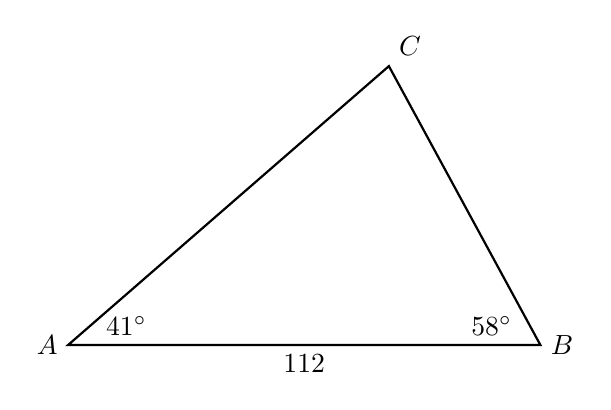
\begin{tikzpicture}[scale=1.2]
      \draw [-, thick] (41:4.5) node[above right]{$C$}--
        (0,0) node[left]{$A$}--
        (5,0) node[right]{$B$}--cycle;
      \node at (0.3, 0)[above right]{$41^\circ$};
      \node at (4.8, 0)[above left]{$58^\circ$};
      \node at (2.5, 0)[below]{$112$};
    \end{tikzpicture}
    \end{center} \vspace{1cm}

\item Find the slant height of a cone with a diameter of 32 centimeters and height of 12 cm. \vspace{1cm}
    
\item Triangle $ABC$ has an area of 100, with $AB=15$ and $AC=17$. Find the measure of the angle $A$. \\[0.5cm]
    Hint: Consider that the two configurations shown have the same base and altitude.
    \begin{flushleft}
      \begin{tikzpicture}[scale=0.3]
        \draw [-, thick] (51.7:17) node[above right]{$C$}--
          (0,0) node[left]{$A$}--
          (15,0) node[right]{$B$}--cycle;
        \node at (1, 0)[above right]{$\theta$};
        \node at (5, 7)[above left]{$17$};
        \node at (8, 0)[below]{$15$};

      \begin{scope}[shift={(35,0)}]
          \draw [-, thick] ({180-51.7}:17) node[above right]{$C'$}--
            (0,0) node[left]{$A'$}--
            (15,0) node[right]{$B'$}--cycle;
          \node at (0, 0)[above right]{$180-\theta$};
          \node at (-5.5, 5)[above left]{$17$};
          \node at (8, 0)[below]{$15$};
      \end{scope}

      \draw [-, dashed] (11.5,13.33)--(24,13.33);

      \end{tikzpicture}
      \end{flushleft} 


\item Express each value as a decimal, first writing the whole calculator display, and then the 3 sig-fig approximation. \hfill [4 marks]
  \begin{multicols}{2}
    \begin{enumerate}
    \item $\displaystyle \frac{2\pi}{3}$
    \item $\displaystyle \frac{\sqrt{3}}{2}$
    \end{enumerate}
  \end{multicols}

\item Express each value as a decimal, rounding to 3 sig-figs if necessary. \hfill [3 marks]
  \begin{multicols}{2}
    \begin{enumerate}
    \item $4.561 \times 10^4$
    \item $1.90 \times 10^{-3}$
    \end{enumerate}
  \end{multicols}

\item Find the volume of a spherical balloon 36 meters in diameter. \hfill [3 marks]
  
\item A cone has a height of 24 cm and volume of $220.5\pi \,\mathrm{ cm}^3$. Find its radius. \hfill [3 marks]
  
\item $\triangle ABC$ is shown with $m\angle C=90^\circ$ and the lengths of the triangle's sides are $BC=8$, $AC=6$, and $AB=10$.
  \begin{multicols}{2}
        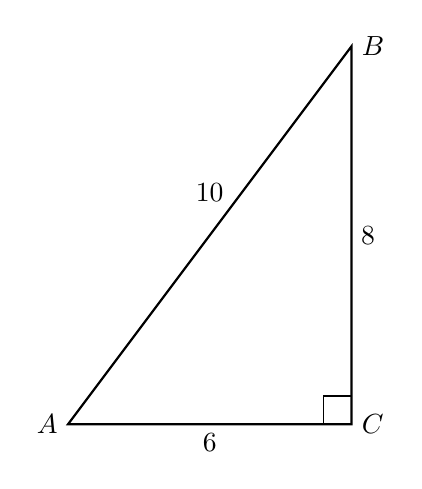
\begin{tikzpicture}[scale=0.6]
          \draw [thick]
          (0,0)node[left]{$A$}--
          (6,0)node[ right]{$C$}--
          (6,8)node[right]{$B$}--cycle;
          \draw (6,0)++(-0.6,0)--++(0,0.6)--+(0.6,0);
          \node at (3,0)[below]{$6$};
          \node at (6,4)[right]{$8$};
          \node at (3,4.5)[above]{$10$};
        \end{tikzpicture}
        \begin{enumerate}
        \item Write down the value of $\sin A$.  \\ \hfill [1 mark]\vspace{1cm}
        \item Find the measure of $\angle A$.  \hfill [2 marks] \vspace{1cm}
      \end{enumerate}
    \end{multicols}

\item In right triangle $ABC$, hypotenuse $\overline{AB}$ has a length of 26 cm, and side $\overline{BC}$ has a length of 17.6 cm. What is the measure of angle $B$?
   
\item Find the slant height of a pyramid with square base 4 meters on a side and height of 4 m. \hfill [3 marks]
    
\item Triangle $ABC$ has an area of 25, with $AB=7$ and $AC=8$. 
   \begin{enumerate}
     \item Find the two possible measures for $\hat{A}$. \hfill [4 marks]
     \item Given that $\hat{A}$ is obtuse, find $BC$. \hfill [3 marks]
   \end{enumerate}

   \newpage

\item The following diagram shows triangle $ABC$ (not drawn to scale).
  \begin{center}
    \begin{tikzpicture}[scale=1.4, rotate=-25]
      \draw [-, thick] (50:3.5) node[above right]{$C$}--
        (0,0) node[left]{$A$}--
        (5,0) node[right]{$B$}--cycle;
      \node at (0.3, 0.15)[right]{$50^\circ$};
      \node at (4.5, 0.3)[above left]{$43^\circ$};
      \node at (3.7, 1.8)[below]{$11$};
    \end{tikzpicture}
    \end{center} 
    $BC=11$, $C\hat{A}B=50^\circ$, and $A\hat{B}C=43^\circ$
    \begin{enumerate}
      \item Find $AC$. \hfill [3 marks]
      \item Find the area of triangle $ABC$. \hfill [3 marks]
    \end{enumerate}

\item The following diagram shows quadrilateral $ABCD$ (not drawn to scale).
  \begin{center}
    \begin{tikzpicture}[scale=1.5, rotate=-20]
      \draw [-, thick] (100:3.5) node[above right]{$D$}--
        (0,0) node[below]{$B$}--
        (-5,0) node[below]{$A$}--cycle;
      \draw [-, thick] (100:3.5) --
      (55:3) node[right]{$C$}--
      (0,0);             
      \node at (58:2.9)[left]{$78^\circ$};
      \node at (50:1.5)[right]{$5.1$};
      \node at (-2.5,-0.2)[below]{$8.0$};
      \node at (78:3.5)[below]{$4.2$};
      \node at (-3,2.2)[below]{$8.3$};
    \end{tikzpicture}
    \end{center} 
    $AB=8.0$, $BC=5.1$, $CD=4.2$, $AD=8.3$, and $B\hat{C}D=78^\circ$
    \begin{enumerate}
      \item Find $BD$. \hfill [3 marks]
      \item Find $A\hat{B}D$. \hfill [3 marks]
    \end{enumerate}

\newpage

\item BMI is a measure of a healthy personal weight, 
  \[\displaystyle BMI = \frac{w}{h^2}\]
    where \\
    $w$ is a person's weight in kilograms, and \\
    $h$ is height in meters
    \begin{enumerate} 
        \item Given a height of 160 cm and weight of 54 kg, find the BMI  \hfill [3 marks]
        \item These measurements are not exact. Assuming the height is between 159-161 cm and weight 53-55 kg, find the bounds of the BMI.  \hfill [4 marks]
      \end{enumerate}


\item Express each value as a decimal, first writing the whole calculator display, and then the 3 sig-fig approximation. \hfill [4 marks]
  \begin{multicols}{2}
    \begin{enumerate}
    \item $\displaystyle \frac{\pi}{6}$
    \item $\displaystyle \frac{\sqrt{2}}{2}$
    \end{enumerate}
  \end{multicols}

\item Express each value as a decimal, rounding to 3 sig-figs if necessary. \hfill [3 marks]
  \begin{multicols}{2}
    \begin{enumerate}
    \item $2.718 \times 10^5$
    \item $6.145 \times 10^{-2}$
    \end{enumerate}
  \end{multicols}

\item Find the volume of a cone 6 centimeters in diameter and 10 cm tall. \hfill [3 marks]
  
\item A round beach ball has a volume of $12348\pi \,\mathrm{ cm}^3$. Find its radius. \hfill [3 marks]
  
\item Find the surface area of a cube with side length 5 cm. \hfill [2 marks]
  
\item $\triangle ABC$ is shown with $m\angle C=90^\circ$ and the lengths of the triangle's sides are $BC=5$, $AC=12$, and $AB=13$. (not drawn to scale)
  \begin{multicols}{2}
        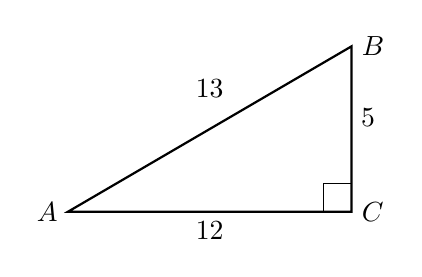
\begin{tikzpicture}[scale=0.6]
          \draw [thick]
          (0,0)node[left]{$A$}--
          (6,0)node[ right]{$C$}--
          (6,3.5)node[right]{$B$}--cycle;
          \draw (6,0)++(-0.6,0)--++(0,0.6)--+(0.6,0);
          \node at (3,0)[below]{$12$};
          \node at (6,2)[right]{$5$};
          \node at (3,2.2)[above]{$13$};
        \end{tikzpicture}
        \begin{enumerate}
        \item Write down the value of $\cos A$.  \\ \hfill [1 mark]\vspace{0.5cm}
        \item Find the measure of $\angle A$.  \hfill [2 marks] \vspace{1cm}
      \end{enumerate}
    \end{multicols}

\item In right triangle $ABC$, hypotenuse $\overline{AB}$ has a length of 19.5 cm, and side $\overline{BC}$ has a length of 12.4 cm. What is the measure of angle $B$? \hfill [3 marks]
  
\item Find the slant height of a cone with radius of 1.5 meters and height of 4 m. \hfill [3 marks]
  
\item Triangle $ABC$ has an area of 22, with $AB=6.5$ and $AC=7.1$. 
  \begin{enumerate}
    \item Find the two possible measures for $\hat{A}$. \hfill [4 marks]
    \item Given that $\hat{A}$ is obtuse, find $BC$. \hfill [3 marks]
  \end{enumerate}

   \newpage

\item The following diagram shows triangle $ABC$ (not drawn to scale).
  \begin{center}
    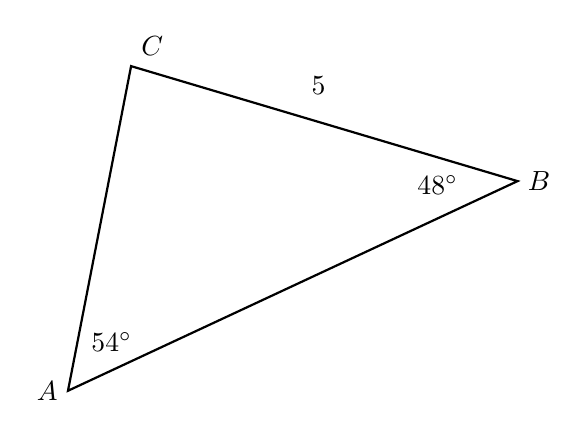
\begin{tikzpicture}[scale=1.4, rotate=25]
      \draw [-, thick] (54:3) node[above right]{$C$}--
        (0,0) node[left]{$A$}--
        (4.5,0) node[right]{$B$}--cycle;
      \node at (0.3, 0.35)[right]{$54^\circ$};
      \node at (4, 0)[above left]{$48^\circ$};
      \node at (3.3, 1.7)[below]{$5$};
    \end{tikzpicture}
    \end{center} 
    $BC=5$, $C\hat{A}B=54^\circ$, and $A\hat{B}C=48^\circ$
    \begin{enumerate}
      \item Find $AC$. \hfill [3 marks]
      \item Find the area of triangle $ABC$. \hfill [3 marks]
    \end{enumerate}

\item The following diagram shows quadrilateral $ABCD$ (not drawn to scale).
  \begin{center}
    \begin{tikzpicture}[scale=1.5, rotate=-30]
      \draw [-, thick] (100:3.5) node[above right]{$D$}--
        (0,0) node[below]{$B$}--
        (-5,0) node[below]{$A$}--cycle;
      \draw [-, thick] (100:3.5) --
      (55:3) node[right]{$C$}--
      (0,0);             
      \node at (58:2.9)[left]{$74^\circ$};
      \node at (50:1.5)[right]{$5.0$};
      \node at (-2.5,-0.2)[below]{$7.8$};
      \node at (78:3.5)[below]{$3.8$};
      \node at (-3,2.2)[below]{$9.1$};
    \end{tikzpicture}
    \end{center} 
    $AB=7.8$, $BC=5.0$, $CD=3.8$, $AD=9.1$, and $B\hat{C}D=74^\circ$
    \begin{enumerate}
      \item Find $BD$. \hfill [3 marks]
      \item Find $A\hat{B}D$. \hfill [3 marks]
    \end{enumerate}

\newpage

\item BMI is a measure of a healthy personal weight, 
  \[\displaystyle BMI = \frac{w}{h^2}\]
    where \\
    $w$ is a person's weight in kilograms, and \\
    $h$ is height in meters
    \begin{enumerate} 
        \item Given a height of 160 cm and weight of 54 kg, find the BMI  \hfill [3 marks]
        \item These measurements are not exact. Assuming the height is between 159-161 cm and weight 53-55 kg, find the bounds of the BMI.  \hfill [4 marks]
      \end{enumerate}

\item The following diagram shows a pole BT 1.6 m tall on the roof of a vertical building. \\[0.25cm]
      The angle of depression from T to a point A on the horizontal ground is  
      $35^\circ$. \\[0.25cm]
      The angle of elevation of the top of the building from A is  
      $30^\circ$. 
        \begin{center}
          \begin{tikzpicture}[scale=0.4]
            %\draw [-, thick] (0,0)--(35:23);
            \draw [-, thick] (-4,0)--
            (0,0)--
              (17,0)--
              (22,0)--
              (22,10)--(17,10) node[left]{$B$};
            \draw [-, thick] (17,0)--(17,12)node[left]{$T$};
            \draw [fill] (0,0) circle [radius=0.1] node[below]{$A$};
            \node at (-3, 0)[below]{ground};
            \node at (19.5, 5)[above]{building};
          \end{tikzpicture}
          \end{center}
          Find the height of the building.  \hfill [7 marks]


\end{enumerate}
\end{document}